\documentclass[fleqn]{article}
\usepackage{lipsum} 
\usepackage{manyeqns}
\usepackage{amsmath}
\setlength{\mathindent}{0.5cm}
\usepackage{soul}
\usepackage{color}
\usepackage{eurosym}
\usepackage{natbib}
\usepackage[sc]{mathpazo} % Use the Palatino font
\usepackage[T1]{fontenc} % Use 8-bit encoding that has 256 glyphs
\linespread{1.05} % Line spacing - Palatino needs more space between lines
\usepackage{microtype} % Slightly tweak font spacing for aesthetics
\usepackage{rotating}
\usepackage[hmarginratio=1:1,top=32mm,columnsep=20pt]{geometry} % Document margins
\usepackage{multicol} % Used for the two-column layout of the document
\usepackage{multirow}
\usepackage{hyperref} % For hyperlinks in the PDF

\usepackage[hang, small,labelfont=bf,up,textfont=it,up]{caption} % Custom captions under/above floats in tables or figures
\usepackage{booktabs} % Horizontal rules in tables
\usepackage{float} % Required for tables and figures in the multi-column environment - they need to be placed in specific locations with the [H] (e.g. \begin{table}[H])

\usepackage{lettrine} % The lettrine is the first enlarged letter at the beginning of the text
\usepackage{paralist} % Used for the compactitem environment which makes bullet points with less space between them

\usepackage{graphicx}
\usepackage[FIGBOTCAP]{subfigure}
\usepackage{multirow, booktabs}

\usepackage{abstract} 
\renewcommand{\abstractnamefont}{\normalfont\bfseries} % Set the "Abstract" text to bold
\renewcommand{\abstracttextfont}{\normalfont\small\itshape}
%\citestyle{nSIE}

\usepackage{titlesec} % Allows customization of titles
\renewcommand\thesection{\Roman{section}}
\titleformat{\section}[block]{\large\scshape\centering}{\thesection.}{1em}{} % Change the look of the section titles


\usepackage{fancyhdr} % Headers and footers
\pagestyle{fancy} % All pages have headers and footers
\fancyhead{} % Blank out the default header
\fancyfoot{} % Blank out the default footer
\fancyhead[C]{Paper for review} % Custom header text
\fancyfoot[RO,LE]{\thepage} % Custom footer text

\begin{document}
	
	\title{\vspace{-5mm}\fontsize{14pt}{10pt}\selectfont\textbf{An Integrated Asset Management Approach for Determination of Optimal Intervention Strategies for Pump Stations}} % Article title
	\author{
		\large
		\textrm{Nam Le$^{a}$}\thanks{Corresponding author: namlt@protonmail.ch} \hspace{2mm}  and \textrm{Hoang Q. Nguyen$^{b}$} and\hspace{2mm}\textrm{J\"{u}rgen Hackl$^{c}$} % Your name
	}
	\date{}
	\maketitle
	
	\textrm{$^{a}$ PhD, Freelancer and Consultant at GHD Ply Ltd.} \\ % Your institution
	\textrm{$^{b}$ Consultant at POM+ Consulting Ltd.} \\ % Your institution
	\textrm{$^{c}$ M.eng, Research Associate, ETH Z\"{u}rich, Switzerland.} \\ % Your institution
	
	\thispagestyle{fancy}
	
	\begin{abstract}
		Pump stations of a water distribution network in Megacities are designed to provide adequate level of services (LOS) of drinking water for millions of city dwellers. If a pump station fails to provide adequate LOS, negative impacts will incur to stakeholders. The revenue and profit generated from selling water for the Water Service Provider (WSP) will be reduced. The people and the public will have less to no water to consume for drinking and usage. Thus, the reliability and efficiency of pump stations are vital. In order to ensure pump stations are reliable, operating with maximum availability and efficiency possible, and with less breakdown, the WSP shall develop a preventive intervention program that consider long-term supply and demand of water and maximizing benefits for the society. 

		This papers proposes an Integrated Asset Management (IAM) Approach to be used to determine optimal intervention strategy for pump stations. The approach is centralized on developing a set of suitable reliability models such as Fault Tree Analysis, hazard deterioration models, block and age replacement models for life cycle cost analysis. 
		
	%	The implementation of the approach requires asset managers to appropriate collect sufficient data over a certain time window
		
		\bigskip
		
		{\bf Keywords:} Integrated Asset Management, Optimal intervention strategy, Hazard Models, Block replacement model, Age Replacement Model, Fault Tree Analysis, Life Cycle Cost Analysis, Pump Stations, Drinking Water.\bigskip
	\end{abstract}
	
	%%%%%%%%%%%%%%%%%%%%%%%%%%%%%%%%%%%%
	
\chapter{Methodology} % Write in your own chapter title
\label{Chapter3}
%\lhead{Chapter 3. \emph{Methodology}} % Write in your own chapter title to set the page header

\section{The Integrated Asset Management Approach (IAM)}
\label{31}
We proposes an Integrated Asset Management (IAM) approach with its framework shown in Figure \ref{iam_pomplus} for executing this project. The IAM approach will eventually be beneficial to Clients as it will lay a foundation to build up a systematic asset management plan for the future. %i.e. we are not only providing the solution to this project but also trying to support Clients in building up a good infrastructure asset management system (IAMS) in the future as we are aware of Client's recent strategic formation of asset management division.

\begin{figure}[!htb]
	%	\begin{center}
	\includegraphics[scale=0.3]{figures/iam_pomplus} 
	%	\end{center}
	\caption{Integrated asset management approach (adopted from POM+  \href{http://www.pomplus.vn}{http://www.pomplus.vn})}

	\label{iam_pomplus}
\end{figure}

As can be seen in Figure \ref{iam_pomplus}, we sees the overall picture of works that should be executed in close connection to each other in order to make a full cycle of asset management effectively. 

Works associated with auditing equipment and facilities of pump stations and reservoirs, coming up with a preventive maintenance program, tendering, and detailed design can be described explicitly using the framework in Figure \ref{iam_pomplus}. For example, various type of data concerning physical and operational condition and performance of equipment and facilities will be collected, filtered, and analyzed (Data Acquisition); the data will be further used for modeling purposes (e.g. prediction of failure rate, draw deterioration curve, reliability and efficiency); life cycle cost analysis will be then performed for each equipment and for its system. In this process, either prioritization or optimization technique can be used; finally a set of preventive maintenance intervention strategies will be generated for decision making purposes.

\section{Deterioration process and rating index}
In order to analyze and forecast the deterioration of assets, it is necessary to accumulate time series data on the CS of the assets. The historical deterioration process of an asset is described in Figure \ref{transitioncs}. This figure shows the deterioration progress of a component that has not been repaired. In reality, there exists uncertainty in the deterioration progress of the asset, and moreover, the CS at each point in the time axis is restricted by the time, at which, visual inspection is carried out. 

In this figure, $\tau$ represents real calendar time (the expression ``time'' will be used instead throughout this paper). The deterioration of the asset starts immediately after it begins to operate at time $\tau_0$. The CS of an asset is expressed by a rank $J$ representing a state variable $i~(i=1,\cdots,J)$. For a component in the good or new situation, its condition state is given as $i=1$, and increasing of CS $i$ describes progressing deterioration. A value of $i=J$ indicates that an asset has reached its service limit. In Figure \ref{transitioncs}, for each discrete time $\tau_i~(i=1,\cdots,J-1)$ on the time-axis, the corresponding CS has increased from $i$ to $i+1$. Hereinafter $\tau_i$ is referred to the time a transition from a CS $i$ to $i+1$ occurs.

\begin{figure}[!htb]
		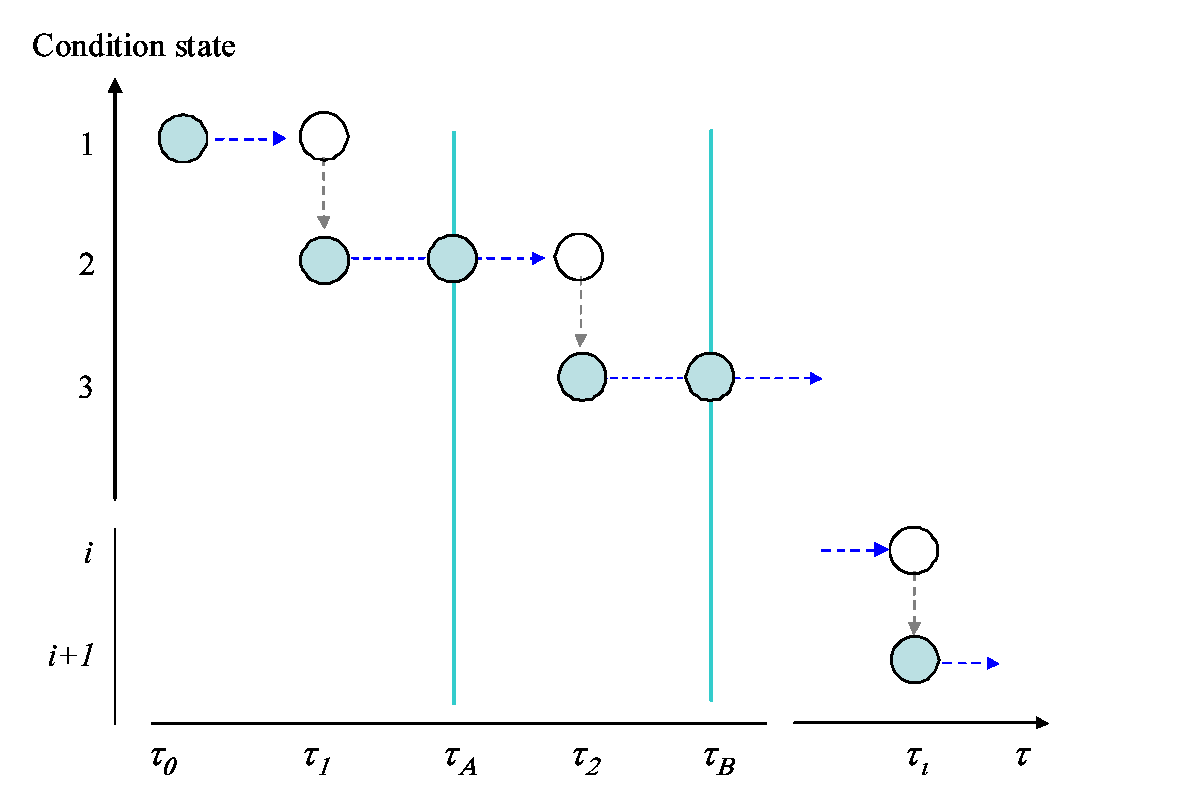
\includegraphics[scale=0.4]{figures/transitioncs.eps} \\
	\footnotesize Note) In this example, the deterioration process of a infrastructure component if expressed in terms of calendar time $\tau_1, \tau_2,...,\tau_i$, and condition state of the section is increased in unitary units.
	\caption{Transition Time of Condition State (adopted from \cite{Lethanh2009c}).}
	\label{transitioncs} 
\end{figure}
%%
%
Information regarding the deterioration process of an asset can be acquired through periodical visual inspections. However, information on the CS based on continuous visual inspection is difficult to obtain. In this case, the initial inspections is carried out at times $\tau_A$ on the time-axis. It is supposed that at time $\tau_A$ the CS observed by inspection is $i~(i=1,\cdots,J-1)$. The deterioration progress in future times is uncertain. Among the infinite set of possible scenarios describing the deterioration process only one path is finally realized. 

Figure \ref{transitioncs01} shows four possible sample paths. Path 1 shows no transition in the CS $1$ from initial time $\tau_0$ to first inspection time $\tau_A$. In paths 2 and 3, CS has advanced to one upper CS at the calendar times $\tau_1^2$ and $\tau_1^3$ respectively. The CS of these two paths observed at time $\tau_A$ become $2$. In a periodical inspection scheme, the point times $\tau_1^2$ and $\tau_1^3$ in which the CS has changed from $1$ to $2$ are not determined. In addition, path 4 shows transitions in the CS at times $\tau_i^4$ and $\tau_{i+1}^4$ during the inspection interval. The CS observed at time $\tau_A$ becomes $3$. That is, in spite of the transitions in the CS are observable at the time of periodical inspection, it is not possible to obtain information about the times in which those transitions occur.

Figure \ref{transitioncs02} further describes the deterioration process inferring the inspection approach and how the CS is assumed. In this figure, it is assumed that the CS at the calendar time $\tau_{i-1}$ has changed from $i-1$ to $i$. The calendar time $\tau_{i-1}$ is assumed to be equivalent to $y_i=0$. The time represented by the sample time-axis is referred from now on as a ``time point'', and differs from ``time'' on the calendar time axis. The times $\tau_A$ and $\tau_B$ correspond to the time points $y_A$ and $y_B$ on the sample axis. It can be seen that $y_A=\tau_A-\tau_{i-1}$, $y_B=\tau_B-\tau_{i-1}$. 

Information on the CS $i$ at the beginning of the calendar time $\tau_{i-1}$ cannot be obtained in a periodical inspection scheme. Therefore, time points $y_A$ and $y_B$ on the sample time-axis cannot be correctly obtained either. For convenience of description, it is assumed that the information at the time a point is known in order to develop the model, despite this assumption is not necessarily essential. The following paragraph discusses that even without information at time points $y_A$ and $y_B$ an exponential hazard model can be estimated.
\begin{figure}[!htb]
		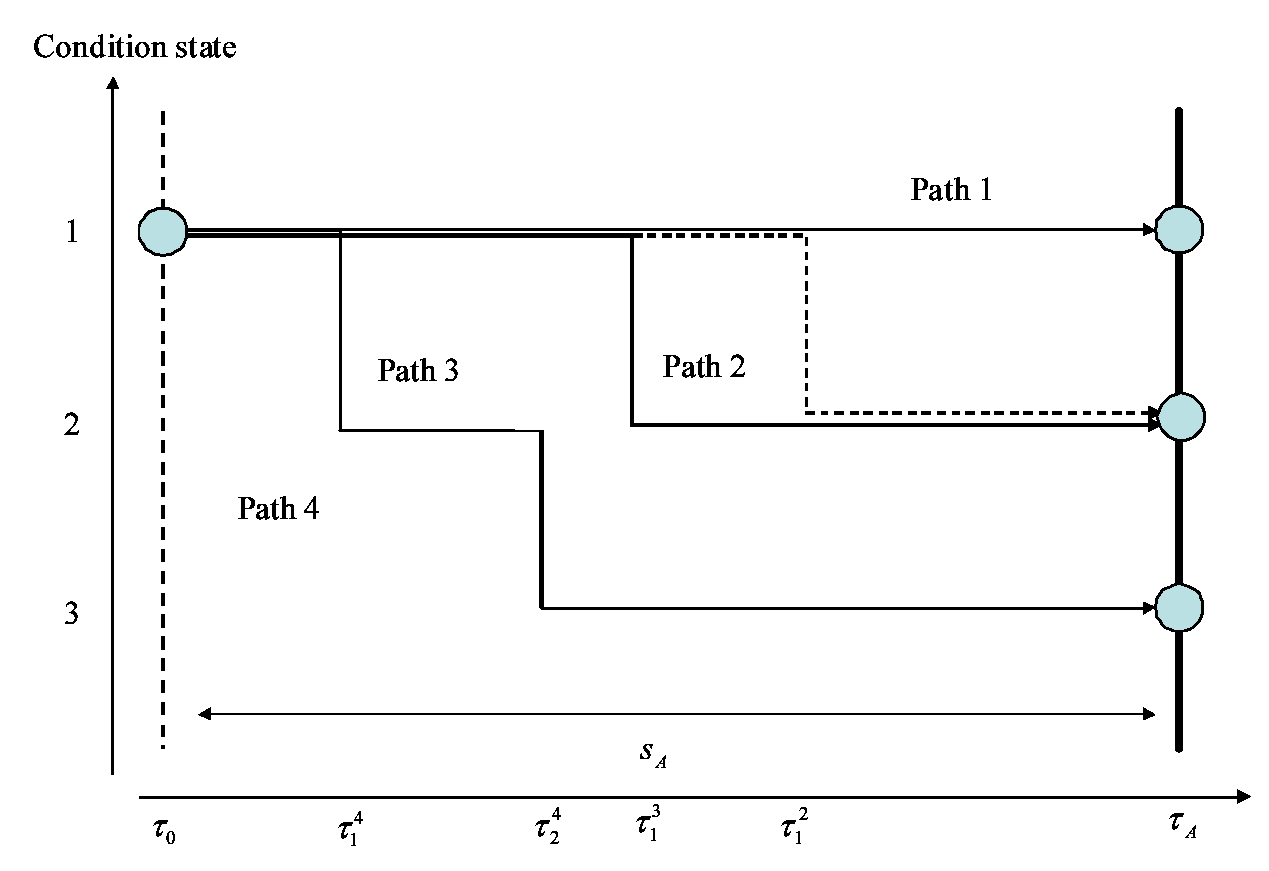
\includegraphics[scale=0.4]{figures/transitioncs01.eps} \\
	\footnotesize Note) In this example, the deterioration process of an asset is expressed in terms of four different sample paths. In paths 2 and 3 the CS has advanced to one upper CS at the calendar times $\tau_1^2$ and $\tau_1^3$ respectively. In path 4, the CS has increased one state at each time $\tau_1^4$ and $\tau_{2}^4$. However, in the case of a periodical inspection carried out at times $\tau_A$ the CS at any point in time between inspections cannot be observed.
	\caption{Transition Pattern of Condition State.}
	\label{transitioncs01} 
\end{figure}

In the case the CS of an asset at time $\tau_{i}$ (time point $y_C$) is assumed to change from $i$ to $i+1$, the period length in which the CS has remained at $i$ (referred as the life expectancy of a CS $i$) is represented by $\zeta_i=\tau_{i}-\tau_{i-1}=y_C$. The life expectancy of a CS $i$ is assumed to be a stochastic variable $\zeta_i$ with probability density function $f_i(\zeta_i)$ and distribution function $F_i(\zeta_i)$. Random variable $\zeta_i$ is defined in the domain $[0,\infty]$. The distribution function is defined as
\begin{eqnarray}
&& F_i(y_i)=\int_0^{y_i}f_i(\zeta_i)d\zeta_i. \label{func21}
\end{eqnarray}
\begin{figure}[!htb]
		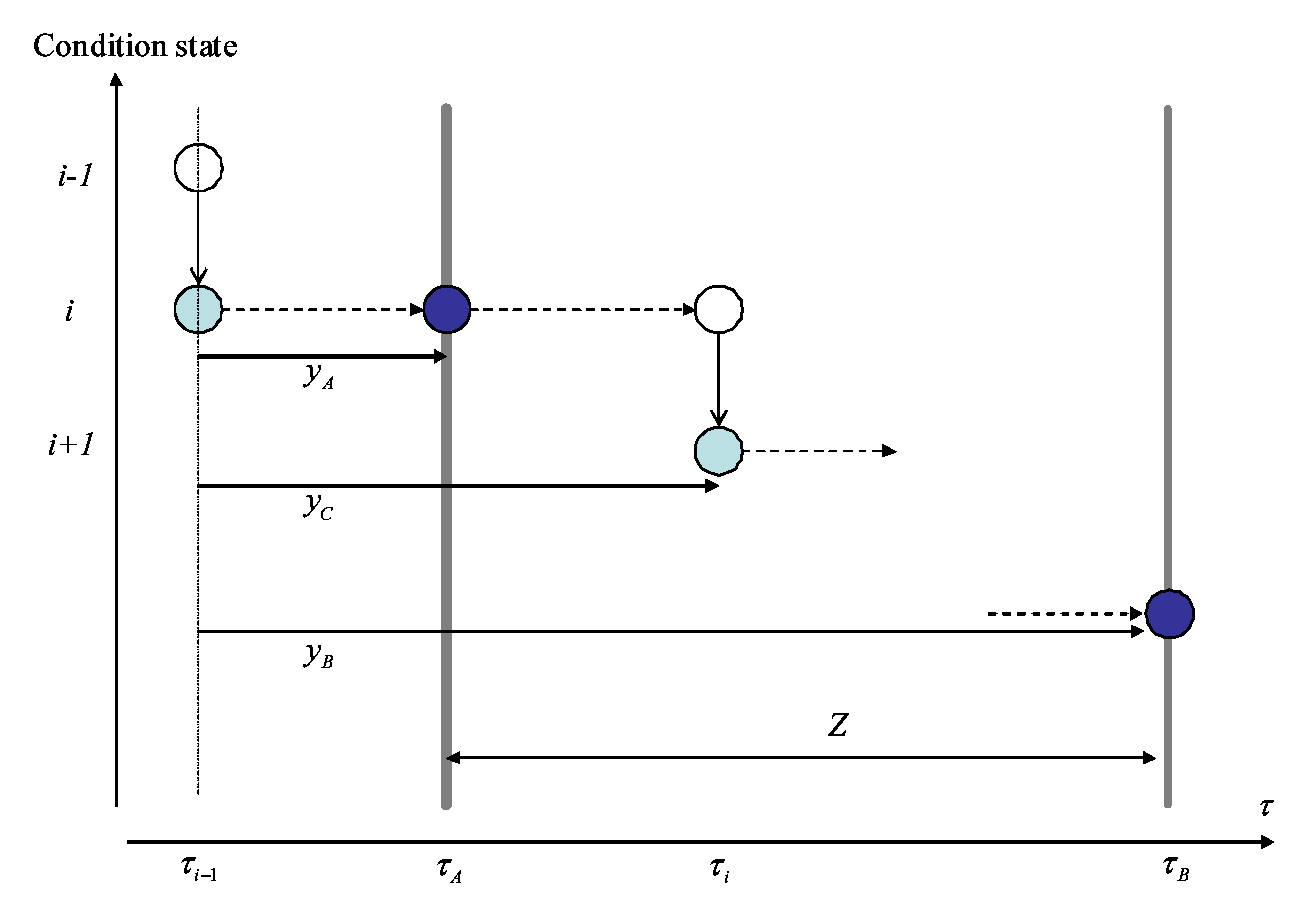
\includegraphics[scale=0.4]{figures/transitioncs02.eps} \\
	\footnotesize Note) In the case the condition state changes from $i-1$ to $i$ at the calendar time $\tau_{i-1}$ the inspections carried out at times $\tau_A$ and $\tau_B$ will also correspond to the points in time $y_A$ and $y_B$ when using $\tau_{i-1}$ as the time origin. The figure shows a sample deterioration path in which the condition state has advanced in one unit to $y_c$ in the interval time $\tau_{i-1}-y_C$. However, observations at time $\tau_{i-1}$ are not possible in a periodical inspection scheme, so there is no way to obtain observation at $y_A$, $y_B$ and $y_C$. Nevertheless, it is possible to use the information contained in $z=y_C-y_A \in [0,Z]$.
	\caption{Model of Deterioration Process.}
	\label{transitioncs02} 
\end{figure}

The distribution function $F_i(y_i)$ represents the cumulative probability of the transition in the CS from $i$ to $i+1$. CS $i$ is assumed to be observed at initial time $y_i=0$(time $\tau_A$). The time interval measured along the sample time-axis until the time point $y_i$ is $\tau_{i-1}+y_i$. Therefore, using the cumulative probability $F_i(y_i)$, the probability $\tilde{F}_i(y_i)$ of a transition in the CS $i$ during the time points interval $y_i=0$ to $y_i\in [0,\infty]$ is defined by $\tilde{F}_i(y_i)$:
\begin{eqnarray}
&& \mbox{Prob}\{\zeta_i \geq y_i\}= \tilde{F}_i(y_i) = 1 -  F_i(y_i). \label{funcbF}
\end{eqnarray}
The conditional probability that the CS of an asset at time $y_i$ advances from $i$ to $i+1$ during the time interval $[y_i,y_i+\Delta y_i]$ is defined as
\begin{eqnarray}
&& \lambda_i(y_i) \Delta y_i = \frac{f_i(y_i)\Delta y_i}{\tilde{F}_i(y_i)}  \label{riskbF},
\end{eqnarray}
where the probability density $\lambda_i(y_i)$ is referred as the hazard function.


\section{Condition State (CS) definition}
\label{csdefinition}
Condition of an asset can be described either by a range of discrete condition state (CS) or by continuous values of one or more than one parameters such as cracking, thickness, and corrosion. In asset management practice, discrete range of CS is often for the following reasons:

\begin{itemize}
	\item It can be converted/mapped from continuous value of monitoring data;
	\item It is convenient for non-technical persons and managers;
	\item It is suitable for determination of intervention strategy and thus for life cycle cost modeling.
\end{itemize}

Assets in pump stations are different in category and functionality, thus it is not easy to define a universal range of CSs. However, it is possible that a generic range of CSs can be used to map appropriately different type of assets. In this project, following definitions are used for multiple CSs (Table \ref{ch03:cs}) and binary state (Table \ref{ch03_csbinary}) systems.


\begin{table}[h]
	\caption{Condition state definition - Multiple.}
	\label{ch03:cs}
	{\footnotesize
\begin{tabular}{l|p{6cm}|l|l}
	\hline
	CS $i$ & Definition & \multicolumn{1}{c|}{Require Intervention} & Remarks \\ 
	\hline
	1 & New/likely new and provide adequate LOS & \multicolumn{1}{c|}{No} & Good (None/Insignificant) \\ 
	2 & Install <=5 years, provide adequate LOS & \multicolumn{1}{c|}{No} & Acceptable (Minor) \\ 
	3 & Moderate aging, not provide adequate LOS, observed moderate breakdown & \multicolumn{1}{c|}{Yes} &  Damaged (Significant)\\ 
	4 & Moderate aging, not provide adequate LOS, require frequent CI and PI & \multicolumn{1}{c|}{Yes} & Poor (Extensive) \\ 
	5 & Aging and not provide adequate LOS & \multicolumn{1}{c|}{Yes} & Safety is endangered  \\ 
	\hline
\end{tabular}
	}
\end{table}

\begin{table}[h]
	\caption{Condition state definition - Binary.}
	\label{ch03_csbinary}
	{\footnotesize
\begin{tabular}{l|p{6cm}|l|l}
	\hline
	\multicolumn{1}{c|}{CS $i$} & Definition & \multicolumn{1}{c|}{Require Intervention} & Remarks \\ 
	\hline
	\multicolumn{1}{c|}{0} & Not provide adequate LOS & \multicolumn{1}{c|}{No} &  \\ 
	\multicolumn{1}{c|}{1} & Provide adequate LOS & \multicolumn{1}{c|}{Yes} &  \\ 
	\hline
\end{tabular}
	}
\end{table}

%Following tables further details definitions of CSs for specific assets in target
%
%\begin{table}[h]
%	\caption{Condition state definition - Valves.}
%	\label{ch03:csvalves}
%	{\footnotesize
%		\begin{tabular}{l|p{6cm}|l|p{3.5cm}}
%			\hline
%			CS $i$ & Definition & \multicolumn{1}{c|}{Require Intervention} & Remarks \\ 
%			\hline
%			1 & New/likely new and provide adequate LOS & \multicolumn{1}{c|}{No} & No leaks and corrosion. Friction in moving parts are not observed \\ 
%			2 & Not new but still provide adequate LOS & \multicolumn{1}{c|}{No} & Acceptable (Minor) \\ 
%			3 & Moderate aging, not provide adequate LOS, observed moderate breakdown & \multicolumn{1}{c|}{Yes} &  Part/s may experience issues with leaks, corrosion, wear or friction but is minor only\\ 
%			4 & Moderate aging, not provide adequate LOS, require frequent CI and PI & \multicolumn{1}{c|}{Yes} & Poor (Extensive) \\ 
%			5 & Aging or not provide adequate LOS & \multicolumn{1}{c|}{Yes} & Valve has deteriorated too much that it fails to function. Failure may be attributed to a particular part or to entirety of valve  \\ 
%			\hline
%		\end{tabular}
%	}
%\end{table}

%
%\begin{table}[h]
%	\caption{Condition state definition - Pipes and fittings.}
%	\label{ch03:csvalves}
%	{\footnotesize
%		\begin{tabular}{l|p{6cm}|l|p{3.5cm}}
%			\hline
%			CS $i$ & Definition & \multicolumn{1}{c|}{Require Intervention} & Remarks \\ 
%			\hline
%			1 & New/likely new and provide adequate LOS & \multicolumn{1}{c|}{No} & No leaks and corrosion. Friction in moving parts are not observed \\ 
%			2 & Not new but still provide adequate LOS & \multicolumn{1}{c|}{No} & Acceptable (Minor) \\ 
%			3 & Moderate aging, not provide adequate LOS, observed moderate breakdown & \multicolumn{1}{c|}{Yes} &  Part/s may experience issues with leaks, corrosion, wear or friction but is minor only\\ 
%			4 & Moderate aging, not provide adequate LOS, require frequent CI and PI & \multicolumn{1}{c|}{Yes} & Poor (Extensive) \\ 
%			5 & Aging or not provide adequate LOS & \multicolumn{1}{c|}{Yes} & Valve has deteriorated too much that it fails to function. Failure may be attributed to a particular part or to entirety of valve  \\ 
%			\hline
%		\end{tabular}
%	}
%\end{table}




\section{Technical efficiency}
\label{32}
Technical efficiency is a coefficient measured as the ratio of actual parameter value and expected/design parameter value. In case of PSs, TE is often discussed around the value of pump efficiency ($\eta$), which is a factor that accounts for the kinetic energy lost during the operation \cite{Girdhar2005}. The PE is a product of the followings:

\begin{itemize}
	\item Hydraulic efficiency (primarily, disk friction against the liquid with impeller shrouds). This efficiency is contributed by the speed and impeller geometry. Shock losses during rapid changes in direction along the impeller and volute can also resulted in additional shock losses;
	\item Volumetric efficiency (recirculation losses at wear rings, interstage bushes and other);
	\item Mechanical efficiency (friction at seals or gland packing and bearings)
\end{itemize}

Hydraulic efficiency and volumetric efficiency are used at the design stage of PS when there is a need to determine suitable pump or group of pumps that satisfies the designed LOS. Whilst, mechanical efficiency is used to determine operational efficiency once pumps are in used.

The mechanical efficiency ($\eta_m$) is estimated based on the equation \ref{HE}

\begin{eqnarray}
&& \eta_p = \frac{P_W}{P_B} \label{HE}
\end{eqnarray}
Where $P_W$ and $P_B$ are water power and brake power, respectively. 

Following equations are used to calculated the $P_W$ and $P_B$:

\begin{eqnarray}
&& P_{W(kW)} = \gamma \times H \times Q \label{PW}
\end{eqnarray}

\begin{eqnarray}
&& P_{B(kW)} = P_E \times e_m \label{PB}
\end{eqnarray}


%hydraulic efficiency
%\begin{eqnarray}
%&& P_{H(kW)} = \frac{Q\times \delta \times g\times H}{3.6\times 10^6} \label{PH}
%\end{eqnarray}

%Motor efficiency
%\begin{eqnarray}
%&& P_{M(kW)} = \frac{\sqrt{3}\times V \times I\times \cos{\phi}\times \theta_e}{1000} \label{PH}
%\end{eqnarray}

where\\
\begin{table}[h]
	\hspace*{1.0cm}
	{\footnotesize
		\begin{tabular}{l|l}
			\multicolumn{1}{c}{$P_W$} & \textit{Water power (kW);}  \\ 
			\multicolumn{1}{c}{$P_B$} & \textit{Brake power (kW);}  \\ 
			\multicolumn{1}{c}{$P_E$} & \textit{Electric power (kW);}  \\ 
			\multicolumn{1}{c}{$Q$} & \textit{Water flow rate ($m^3/s$);}  \\ 
			\multicolumn{1}{c}{$H$} &\textit{ Head produced by pump ($m_{H_2O}$);}\\ 
			\multicolumn{1}{c}{$\eta_e$} &\textit{Motor efficiency (\%); } \\			
			\multicolumn{1}{c}{$\gamma$} &\textit{specific weight of fluid (water) ($kN/m^3$). } \\						
		\end{tabular}
	}
\end{table}


%\begin{table}[h]
%	\hspace*{1.0cm}
%	{\footnotesize
%%		\begin{tabular}{l|l}
			%\multicolumn{1}{c}{$Q$} & \textit{Differential head;}  \\ 
			%\multicolumn{1}{c}{$\delta$} & \textit{Volumetric flow ($m^3/h$);}  \\ 
			%\multicolumn{1}{c}{$g$} &\textit{Density at pump temperature ($kg/m^3$); } \\ 						
			%\multicolumn{1}{c}{$H$} &\textit{ Gravitational acceleration - $9.81 m/s^2$; } %\\ 									
%			\multicolumn{1}{c}{$V$} &\textit{ Measured voltage in volts; } \\ 									
%			\multicolumn{1}{c}{$I$} &\textit{ Measured current in ampere; } \\
%			\multicolumn{1}{c}{$\cos\phi$} &\textit{ Measured power factor; } \\			
%			\multicolumn{1}{c}{$\eta_e$} &\textit{Motor efficiency. } \\			
%		\end{tabular}
%	}
%\end{table}


\section{Reliability}\label{33}
\subsection{Qualitative and Operational Analysis}
%The methodology employed is Reliability Centered-Maintenance (RCM). The concept entails a thorough periodic study of the plant systems operations and maintenance procedure. For this project, the concept of Standby Unit Philosophy will be utilized for the Maintenance Program that will be proposed. This philosophy revolves around the concept of having a dedicated duty and dedicated spare pump. The maintenance policy for Duty Pump (A) could be RUN TO FAILURE or minimal monitoring only and the focus of maintenance will then be on the reliability of Standby Pump (B).
\subsubsection{Failure Mode and Effects Analysis (FMEA)}
An FMEA is often the first step of a system reliability study. It involves reviewing as many components, assemblies, and subsystems as possible to identify failure modes, and their causes and effects.  
FMEA is an inductive reasoning (forward logic) single point of failure analysis and is a core task in reliability engineering, safety engineering and quality engineering.

A successful FMEA activity helps identify potential failure modes based on experience with similar products and processes—or based on common physics of failure logic. It is widely used in development and manufacturing industries in various phases of the product life cycle. 

Functional analyses are needed as an input to determine correct failure modes, at all system levels. The FMEA is in principle a full inductive (forward logic) analysis, however the failure probability can only be estimated or reduced by understanding the failure mechanism. Hence, FMEA may include information on causes of failure (deductive analysis) to reduce the possibility of occurrence by eliminating identified (root) causes.

\subsubsection{Reliability Centered Maintenance (RCM) }
Reliability-centered maintenance (RCM) is a process to ensure that systems continue to do what their user require in their present operating context. It is generally used to achieve improvements in fields such as the establishment of safe minimum levels of maintenance. Successful implementation of RCM will lead to increase in cost effectiveness, reliability, machine uptime, and a greater understanding of the level of risk that the organization is managing. It is defined by the technical standard SAE JA1011, Evaluation Criteria for RCM Processes.

Reliability centered maintenance is an engineering framework that enables the definition of a complete maintenance regimen. It regards maintenance as the means to maintain the functions a user may require of machinery in a defined operating context. As a discipline it enables machinery stakeholders to monitor, assess, predict and generally understand the working of their physical assets. This is embodied in the initial part of the RCM process which is to identify the operating context of the machinery, and write a Failure Mode Effects Analysis (FMEA). The second part of the analysis is to apply the "RCM logic", which helps determine the appropriate maintenance tasks for the identified failure modes in the FMEA. Once the logic is complete for all elements in the FMEA, the resulting list of maintenance is "packaged", so that the periodicities of the tasks are rationalised to be called up in work packages; it is important not to destroy the applicability of maintenance in this phase. Lastly, RCM is kept live throughout the "in-service" life of machinery, where the effectiveness of the maintenance is kept under constant review and adjusted in light of the experience gained.

RCM can be used to create a cost-effective maintenance strategy to address dominant causes of equipment failure. It is a systematic approach to defining a routine maintenance program composed of cost-effective tasks that preserve important functions.






\subsection{Fault Tree Analysis (FTA)}
Fault Tree Analysis (FTA) is a logical and graphical method to represent the chain of events leading to failure of system \cite{Larsen1974, Pate-Cornell1984}. The method has been used widely for assessment of reliability of industrial and nuclear power plants. It has been proved to be a suitable approach to identify critical assets of a plant that require special attention. 

A set of representative FTA graphs for a typical pump station is illustrated in this subsection.

\begin{figure}[!htb]
	\includegraphics[scale=1.3]{figures/fta01} \\
	\caption{Fault Tree - Causes of Failure}
	\label{fta01} 
\end{figure}

\begin{figure}[!htb]
	\includegraphics[scale=1.3]{figures/fta02} \\
	\caption{Fault Tree - Failure of Power System}
	\label{fta02} 
\end{figure}

\begin{figure}[t]
	\includegraphics[scale=1.3]{figures/fta03} \\
	\caption{Fault Tree - Failure of Pump System}
	\label{fta03} 
\end{figure}



\subsection{Herz model}
Herz model is a semi-probabilistic model that has been used widely in deterioration prediction of water pipe \cite{Herz1996, Herz1996a, Herz1998}. Following formula describes formula to estimate the proportion or percentage of pipe ($y_i$) that remain in CS $i$ at time $x$.

\begin{eqnarray}
&& y_i(x)=\left\{
\begin{array}{ll}
\frac{a+1}{a+e^{b(x-c)}} & x \geq c\\
1,0 & \text{Otherwise}
\end{array}
\right.
\end{eqnarray}

where\\
\begin{table}[h]
	\hspace*{1.0cm}
	{\footnotesize
		\begin{tabular}{l|l}
			\multicolumn{1}{c}{$a$} & \textit{Deterioration factor;}  \\ 
			\multicolumn{1}{c}{$b$} & \textit{Transition parameter;}  \\ 
			\multicolumn{1}{c}{$c$} &\textit{ Resistance period. } \\ 						
		\end{tabular}
	}
\end{table}

The percentage of CS $i$ remains within a period $x$ is analogy to reliability of the pipe staying in respective CS. The parameters $a$, $b$, and $c$ are calibrated based on historical monitoring data. Thus, having historical data is pre-requisite for applying the model.



\subsection{Weibull model} \label{ch03:weibullmodel}

In hazard analysis, the deterioration of element is subjected to follow a stochastic process \cite{lancaster90}. For binary state system, two condition level $0, 1$ are often used. When receiving a PI or CI, the CS from $1$ must be changed into $0$. In reliability study, this process is often regarded as renewal process. The renewal is carried out at alternative time $t_k$ $(k=0,1,2,...)$. In this way, the next renewal time is denoted as $t=t_0+\tau$, where $\tau$ indicating the elapsed time. The life span of an asset is expressed by a random variable $\zeta$. The probability distribution and probability density function of the failure occurrence are $F(\zeta)$ and $f(\zeta)$ respectively. The domain of the random variable $\zeta$ is $[0,\infty]$. The living probability (hereafter named as survival probability) expressed by survival function $\tilde{F}(\tau)$ can be defined according to the value of failure probability $F(\tau)$ in the following equation:

\begin{eqnarray}
&& \tilde{F}(\tau) = 1 - F(\tau). \label{funcbF5}
\end{eqnarray}
The probability, at which the asset performs in good shape until time $\tau$ and break down for the first time during an interval of $\tau+\Delta\tau$ can be regarded as hazard rate and expressed in the following equation:
\begin{eqnarray}
&& \lambda_i(\tau) \Delta \tau = \frac{f(\tau)\Delta \tau}{\tilde{F}(\tau)}, \label{riskbF5}
\end{eqnarray}
where $\lambda(\tau)$ is the hazard function of the asset. In reality, the breakdown probability depends largely on the elapsed time of the asset since its beginning of operation. Thus, the hazard function should take into account the working duration of the asset (time-dependent). In another word, the memory of the system should be inherited. Weibull hazard function is satisfied in addressing the deterioration process \cite{Dodson2006, Kobayashi2010a}:
\begin{eqnarray}
&& \lambda(\tau)= \alpha m \tau^{m-1}, \label{weibul}
\end{eqnarray}
where $\alpha$ is the parameter expressing the arrival density of the asset, and $m$ is the acceleration or shape parameter. The probability density function $f(\tau)$ and survival function $\tilde{F}(\tau)$ in the form of Weibull hazard function can be further expressed in equation (\ref{pdf}) and (\ref{survival}):
\begin{eqnarray}
&& f(\tau)=\alpha m\tau^{m-1}\exp(-\alpha \tau^m), \label{pdf} \\
&& \tilde{F}(\tau)=\exp(-\alpha \tau^m). \label{survival}
\end{eqnarray}

Estimation for Weibull's parameter is often with Maximum Likelihood Estimation (MLE) approach on historical data. Thus, the model's parameter is sensitive to how data behaves. We recommend to use this model only when there is sufficient data to be used.

An example of source code for education purpose is given in Github site of Nam Le \footnote{\href{https://github.com/namkyodai/Models}{https://github.com/namkyodai/Models}}. The complete program is a copyright of Nam Le. 

\subsection{Markov model}
\label{232}
The transition process among the condition states of an infrastructure component is uncertain. Therefore, future condition states cannot be forecasted deterministically. In this situation, Markov transition probability is employed to represent the uncertain transition pattern of the condition states during two time points. Markov transition probabilities can be defined for arbitrary time intervals. 

For simplification, Markov transition probabilities can be defined and used to forecast the deterioration of a infrastructure component based on the information from periodical inspection scheme shown in Figure \ref{transitioncs02}. The observed condition state of the component at time $\tau_A$ is expressed by using the state variable $h(\tau_A) $. If the condition state observed at time $\tau_A$ is $i$, then the state variable $h(\tau_A)=i$. A Markov transition probability, given a condition state $h(\tau_A) =i$ observed at time $\tau_A$, defines the probability that the condition state at a future time ($\tau_B$ for example) will change to $h(\tau_B) =j$:
\begin{eqnarray}
&& \mbox{Prob}[h(\tau_B)=j|h(\tau_A)=i]=\pi_{ij}.\label{pro}
\end{eqnarray}
The Markov transition probability matrix can be defined and rearranged by using the transition probabilities between each pair of condition states $(i,j)$ as
\begin{eqnarray}
&& {\bf \Pi}=\left(
\begin{array}{ccc}
\pi_{11} & \cdots & \pi_{1J} \\
\vdots & \ddots & \vdots \\
0 & \cdots & \pi_{JJ}
\end{array}
\right). 
\end{eqnarray}
The Markov transition probability (\ref{pro}) shows the transition probability between the condition states at two given times $\tau_A$ and $\tau_B$, therefore, it is straightforward that the values of a transition probability will differ for different time intervals. Since deterioration continues as long as no repair is carried out $\pi_{ij}=0~(i>j)$. From the definition of transition probability $\sum^{J}_{j=1}\pi_{ij}=1$. Following conditions must be satisfied:
\begin{eqnarray}
\left.
\begin{array}{l}
\pi_{ij}\geq 0 \\
\pi_{ij}=0 \,\,~(\,\mbox{when} \,\,\, i>j) \\
\sum_{j=1}^J \pi_{ij}=1 \\
\end{array}
\right\}.\label{suii}
\end{eqnarray}
The worse level of deterioration is expressed by the condition state $J$, which remains as an absorbing state in the Markov chain as long as no repair is carried out. In this case $\pi_{JJ}=1$.

Markov transition probabilities are defined independently from the deterioration history. As shown in Figure \ref{transitioncs02}, the condition state at the inspection time $\tau_A$ is $i$, however, the time, at which, condition state changed from $i-1$ to $i$ is unobservable. In a Markov chain model, it is assumed that the transition probability between the inspection times $\tau_A$ and $\tau_B$ is only dependent on the condition state at time $\tau_A$. 

The Markov chain model is operative and widely applied in management of infrastructure system. Particularly, at management of network level, Markov chain model is used to define the average transition probability of the entire system, or a group of infrastructure components given two periodical inspection data.

Estimation for the Markov transition probability can be done by the MLE approach \cite{lancaster90, Lethanh2009c} or Bayesian Estimation approach \cite{jeffgill, Kobayashi2012} based on historical data. One advance of using the Markov model is that one time monitoring data can be used. A generic formula to estimate the transition probability is given in following Equations: 

\begin{manyeqns}
	&& \pi_{ii}=\exp(-\theta_i Z), \label{p1} \\
	&& \pi_{ii+1}= \frac{\theta_i}{\theta_{i}-\theta_{i+1}}\{-\exp(-\theta_{i}Z)+\exp(-\theta_{i+1}Z)\}, \\
	&& \pi_{ij}= \sum_{k=i}^{j}\prod_{m=i}^{k-1}\frac{\theta_m}{\theta_{m}-\theta_{k}}\prod_{m=k}^{j-1}\frac{\theta_m}{\theta_{m+1}-\theta_{k}}\exp(- \theta_{k} Z) \label{hazardpiij}, \\
	&& \pi_{iJ}=1-\sum_{j=i}^{J-1}\pi_{ij}, \label{pj}\\
	&& \hspace{5mm} (i=1,\cdots,J-1) \hspace{5mm} (j=i,\cdots,J). \nonumber
\end{manyeqns}

An example of source code for education purpose is given in Github site of Nam Le \footnote{\href{https://github.com/namkyodai/Models}{https://github.com/namkyodai/Models}}. The complete program is a copyright of Nam Le.


\section{Intervention Strategy (IS)}
\label{isntrategy}
Intervention Strategy (IS) is at asset level (level 7). It is a collection of intervention type for component level (level 8). A collection of ISs will form an Intervention Program for (IP) the station. A collection of IPs will form a Work Program (WP) for network level intervention (e.g. a bid awarded for a designer/contractor can be a WP that consists of intervention program for one or more than one pump stations). Following generic IS is defined to guide the selection of IPs that will be details in the later part of the report.

\begin{table}[h]
	\caption{Generic intervention strategy (IS).}
	\label{ch03:is}
	{\footnotesize
		\begin{tabular}{l|p{6cm}|p{6cm}}
			\hline
			IS & Definition &  Remarks \\ 
			\hline
			1 & Do Nothing &   \\ 
			2 & Minor repair  & Require minimal effort and can be done only for certain asset type \\ 
			3 & Major repair  & Require extensive efforts to return the asset to likely new condition \\ 
			4 & Replacement/Renewal  & Replacing assets or components of asset with identical one or with new model \\ 
			\hline
		\end{tabular}
	}
\end{table}

For each type of asset, IS will be selected based on reliability study and consideration of cost. Further more, Employers inputs and requirements are also taken into account.

\section{Determination of optimal intervention strategy}
\label{35}
Following subsections briefly describe the model that can be used to determine optimal intervention strategy. 
\subsection{Block Replacement Model} \label{blockreplace}
It is assumed that a PI is executed after a pre-defined time $n\cdot T$ ($n=0,1,2,\cdots,N$). Once the PI is executed, the functionality and serviceability of the asset could be the same or different from that of the asset before the intervention. In between the time $\Delta t$ ($[0\le \Delta t \le T]$), hazards could occur and cause the asset in worse CSs (hereafter denoted as $i$ ($i=1,\cdots,I$)), in which the asset is no longer providing an adequate level of services (LOS). In both cases, when the PI or CI is executed, there are impacts incurred by stakeholders $s$ (e.g. the owner, the users, the public).

Following notations are used to describe the formulation of the model.


\begin{tabular}{lp{12.5cm}}
	$\theta(\Delta t|t)$ & Conditional failure rate $i$ $(i=1,\cdots,I)$ when the asset has been in service in an interval $t$ after the PI \\ 
	$\Psi(\cdot|t)$ & Any conditional function $\Psi$ given that a PI is executed by a unit of age $t$, where $t$ is a random variable \\ 
	$F(t)$ & Cumulative distribution function (cdf) of age $t$ of a unit for a PI at execution time\\ 
	$w_{p}^s(t)$ & Impacts incurred by stakeholder $s$ due to the execution of PI\\ 
	$w_{c}^s(t)$ & Impacts incurred by stakeholder $s$ due to the execution of CI \\ 
	$w_o^s(\Delta t|t)$ & Conditional impacts incurred by stakeholder $s$ when the structure is remains in normal operation (\emph{i.e.} providing an adequate LOS) during time interval $\Delta t$ after a PI has been carried out and the asset has not entered failure state\\ 
	$\rho$ & discount factor\\
	$p_l^k (t)$ & probability of failure at time $t$ of the affecting other assets $k$ \\
	$C_c^{s,k}$ & Impacts incurred by stakeholder $s$ due to the execution of an CI on other assets $k$ \\
	$T$ & interval between the PIs\\ 
	$T^{\star}$ & Optimal interval time between PIs, which is the variable of the model\\
	$\Omega_{p}(T,t)$ & minimum expected total discounted impact for an infinite time span when the asset has been in service during an interval $t$ after the execution of the PI and the asset has not entered failure state\\
	$\Omega_{c}(T,t)$ & minimum expected total discounted impact for an infinite time span when a CI has been executed, of the asset that has been in service during a time interval $t$ after the execution of the PI and the asset has entered failure state\\
\end{tabular}
In the model, it is assumed that at each damage level $i$, there exists a corresponding well defined CI. Within an increment of time $\Delta t$, after the asset has been under the PI after time $t$, the total expected impacts due to the execution of CIs are:
\begin{eqnarray}
&& v_c (\Delta t|t) =\sum_{s=1}^{S} \left [ w_{c}^s  (\Delta t) + \sum_{k=1}^K p_l^k \cdot C_c^{s,k} \right ] \cdot \theta (\Delta t|t) .\label{totalCIs}
\end{eqnarray}
The total impacts due to the execution of PIs and the total impacts incurred by stakeholders during the service time of the asset are defined in Eq. (\ref{totalPIs}) and Eq. (\ref{totalO}), respectively.
\begin{eqnarray}
&& v_p (t) =\sum_{s=1}^{S}w_{p}^s (t)  .\label{totalPIs}
\end{eqnarray}
\begin{eqnarray}
&& v_o (t) =\sum_{s=1}^{S}w_{o}^s (t)  .\label{totalO}
\end{eqnarray}
According to the principle of optimality, which is described in \cite[p. 15]{Bellman1962}, the minimum expected total discounted impact $\Omega_{c}(T,t)$ for infinite time is formulated in following equation.
\begin{eqnarray}
&& \Omega_{c}(T,t) = \int_0^{\infty} \left[ {v_c(\Delta t|t)} + \Omega_{p}(T,\Delta t|t)  \right] dF(t).\label{omegaCI1}
\end{eqnarray}
The minimum expected total discounted impact $ \Omega_{p}(T,\Delta t|t) $, which appears inside Eq. (\ref{totalCIs}), is obtained as follows
\begin{eqnarray}
&& \Omega_{p}(T,\Delta t) = min \Gamma (\Delta t) .\label{omegaPI1}
\end{eqnarray}
where $\Gamma (\Delta t)$ is defined as
\begin{eqnarray}
&& \Gamma (\Delta t) = \int_0^{\infty} \left[ v_o \int_0^{dt} exp(-\rho \tau)d\tau  + \left\{ {1-\theta(\Delta t|t)dt} \right\}\cdot \Omega_p(T,\Delta t+dt|t) exp(-\rho dt) \right. \nonumber \\
&&  \hspace{20mm} +  \theta(\Delta t|t)dt \cdot \Omega_c(T,\Delta t+dt|t)exp(-\rho dt) \left.\vphantom{\int_t} \right] dF(t).\label{gamma1}
\end{eqnarray}
According to \cite{Kaio1984}, Eq. (\ref{gamma1}) is rewritten in following form
\begin{eqnarray}
&& \Gamma (\Delta t) = \Omega_{p}(T,\Delta t) + \left[ -\rho \Omega_{p}(T,\Delta t) +d\Omega_{p}(T,\Delta t)/dt \right]dt \nonumber \\
&& \hspace{30mm} + \int_0^{\infty} \left[ v_o + v_c(\Delta t|t) \right]dF(t)dt.\label{gamma2}
\end{eqnarray}
Thus, from $\Omega_p(T,\Delta t)=\Gamma(\Delta t)$ (Eq. (\ref{omegaPI1})), the following equation can be derived:
\begin{eqnarray}
&& \Omega_p(T,\Delta t) = exp(\rho\Delta t) \left[\Omega_p(T,0)-\int_0^{\infty}\int_0^t exp(-\rho\tau) \left\{ v_o+v_c(\tau|t)\right\} \right]d\tau dF(t)
.\label{omegaPI2}
\end{eqnarray}
where,
\begin{eqnarray}
&& \Omega_p(T,0) = \left\{1-exp(-\rho T)\right\}^{-1} \int_0^{\infty} \left[ \vphantom{\int_t} exp(-\rho T) \left\{ v_p(T,t) \right\} \right. \nonumber \\
&& \hspace{45mm}+ \int_0^T exp(-\rho \Delta t) \left\{ v_o (\Delta t|t) + v_c(\Delta t|t) \right\} dt \left.\vphantom{\int_t} \right] dF(t).\label{omegaPI3}
\end{eqnarray}
when $T$ tends to infinity $T \to \infty $, Eq. (\ref{omegaPI3}) becomes
\begin{eqnarray}
&& \Omega_p(\infty,0) = \int_0^{\infty}\int_0^{\infty}exp(-\rho t) \left[v_o + v_c(\Delta t|t) \right] dt dF(t).\label{omegaPI4}
\end{eqnarray}
Eqs. (\ref{omegaPI3}) and (\ref{omegaPI4}) are the explicit forms of the expected total discounted impact in infinite time horizon. This is the classical optimization problem. By differentiating the expected total discounted impact $\Omega_p(T,0)$ and $\Omega_p(\infty,0)$ and setting it equal to zero, the optimal time $T^{\star}$ can be obtained. 
The optimal time $T^{\star}$ for PI is the solution of the following system of equations:
\begin{eqnarray}
&& \left\{ {\begin{array}{*{20}{c}}
	{{T^{\star}} = \arg \mathop {\min }\limits_{{T^{\star}} \in [0,T]} {\Theta _p}(T,0)}\\
	{{T^{\star}} = \arg \mathop {\min }\limits_{{T^{\star}} \in [0,\infty ]} {\Theta _p}(\infty ,0)}
	\end{array}} \right. 
\end{eqnarray}
in which the differentiates of $\Theta_p(T,0)$ and $\Theta_p(\infty,0)$ are respectively:
\begin{eqnarray}
&& \Theta_p(T,0)  = \frac{\delta (\Omega_p(T,0))}{\delta T} \nonumber \\
&& \hspace{14mm} = \left[1-exp(-\rho T) \right] \int_0^{\infty} \left[ \vphantom{\int_t} -\rho v_p(T,t) \right. \nonumber \\
&& \hspace{20mm} +d(v_p(T,t))/dT + v_o(T,t) + v_p(T,t) \left.\vphantom{\int_t}\right]dF(t) \nonumber \\
&& \hspace{20mm} -\rho \int_0^{\infty} \left[ \vphantom{\int_t} exp(-\rho T)\left\{v_p(T,t) \right\}\right. \nonumber \\
&& \hspace{20mm}  +\int_0^T exp(-\rho \Delta t) \left\{v_o(\Delta t|t) + v_c(\Delta t|t) \right\} dt \left.\vphantom{\int_t}\right] dF(t).\label{omegaPI5}
\end{eqnarray}
and
\begin{eqnarray}
&& \Theta_p(\infty,0)  = \frac{\delta (\Omega_p(\infty,0))}{\delta T} \nonumber \\
&& \hspace{14mm} = \int_0^{\infty} \left[-\rho \left\{v_p(\infty|t)+ \int_0^{\infty}exp(-\rho t) \left\{v_o(\Delta t|t)+ v_p(\Delta t|t)  \right\}\right\} \right. \nonumber \\
&& \hspace{20mm} + \mathop {\lim }\limits_{T \to \infty } d(v_p(T,t))/dT + v_o(\infty|t) + v_p(\infty|t) \left.\vphantom{\int_t}\right] dF(t) \label{omegaPI6}
\end{eqnarray}

\subsection{Time-dependent replacement model}
Time-dependent replacement model (or Age replacement model) are the ones where the following conditions apply:
\begin{itemize}
	\item the asset starts operating at $t=0$, i.e. it is newly built or newly restored to a like new condition following an intervention;
	\item the probability of failure is described with $f(t)$ and $F(t)$, i.e. the lifetime density and the lifetime;
	\item if the asset fails on the interval $(0,T]$ a CI is executed;
	\item if the object does not fail on the interval $(0,T]$ the object is replaced at $T$, i.e. the PI replacement is executed, regardless if the object has failed and been restored in the time interval $(0,T]$;
	\item the execution of a PI restores the object to a like new condition;
	\item the execution of a CI restores the object to a like new condition.
\end{itemize}
\subsubsection{Minimize impact}
If an age replacement IS is followed the time to the first intervention, Z, is the minimum amount of the time to failure of the length of the renewal period:
\begin{eqnarray}
&& Z=min(\tau,T)
\end{eqnarray}
The expected, or mean, time to the first intervention is then determined by
\begin{eqnarray}
&& E[Z=\int_{0}^{T}(1-F(x))dx]
\end{eqnarray}
The mean impact in one renewal period then equals the probability of failure on $T$ multiplied by the impacts associated with the CI plus the probability that no failure occurs on $T$ multiplied by the impacts associated with the PI:
\begin{eqnarray}
&& F(T)\times I^{CI}+(1-F(T))\times I^{PI}
\end{eqnarray}
The mean impacts per unit time, therefore, equal the mean cost in one renewal period divided by the length of the renewal period, i.e. the time to the first intervention.
\begin{eqnarray}
&& \eta_{AC}=\frac{F(T)\times I^{CI}+(1-F(T))\times I^{PI}}{\int_{0}^{T}(1-F(x))dx]}
\end{eqnarray}
\subsubsection{Maximize availability}
If it is desired to determine the age replacement IS that maximizes availability the following is often assumed, additionally that:
\begin{itemize}
\item the PI replacement takes $t^{PI}$;
\item the PI takes $t^{CI}$;
\end{itemize}
If the asset fails before $T$ then the length of the renewal period will, therefore, be $X=t+t^{CI}$, which has the probability $f(t)dt$ of occurring, and if the object does not fail before $T$ then the length of the renewal period will be $X=t+t^{PI}$, which has the probability $1-F(T)$ of occurring.

In this case, the expected, or mean, renewal period length is:

\begin{eqnarray}
&& E[X] = \int_{0}^{T}(1-F(x))dx + t^{CI}F(T)+t^{PI}(1-F(T))
\end{eqnarray}
As the asset is operational on average $\int_{0}^{T}(1-F(x))dx$ then the availability is given by:
\begin{eqnarray}
&& \eta_{AA} = \frac{\int_{0}^{T}(1-F(x))dx}{\int_{0}^{T}(1-F(x))dx + t^{CI}F(T)+t^{PI}(1-F(T))}
\end{eqnarray}

\section{Return on Investment (ROI)}
Return on Investment (ROI) is a simple way to determine if the investment is worth to be executed. The ROI is defined using the ratio between the Net Profit and the Total Investment.
\begin{eqnarray}
&& ROI = \frac{\text{Net Profit}}{\text{Total Investment}}\times 100
\end{eqnarray}
The Total Investment is referred as CAPEX or ballpark estimate, which can be spent when the IS is executed. In this case, we can assume that the IS will be executed at time 0. This does not mean that the execution falls exactly this year but can be in any year within the planning horizon (e.g. 5 years).

Net Profit is calculated based on Cash Flow Analysis (CFA) that will incorporate the yearly production and resource consumption of the PS (e.g. power, lubricant, chemical). The conventional CFA is done with Net Present Value (NPV)

\begin{eqnarray}
&& NPV = \sum_{t=0}^{T} \left[B(t) - C(t)\right]\times \frac{1}{(1+\rho^t)}
\end{eqnarray}
Where $B(t)$ and $C(t)$ are benefit and cost, respectively. The benefit can be a sum of revenue, profit, and added value for stakeholers, whilst the cost is a sum of CAPEX, operational cost, and other impacts incurred to stakeholders that can be quantified as monetary units.

We suggests the WSPs to consider the 3Rs in applying the above formulas. The 3Rs are revenue, reputation, and regulatory. Revenue can be conveniently estimated. However, reputation and regulatory are hard to quantify. 
	
	\bibliographystyle{plainnat} 
	%\bibliographystyle{unsrt} 
	\bibliography{plantaudit}


	
	%%%
\end{document}




